\chapter{Contexto tecnológico}

En este apartado se describirá, de manera sencilla, diversas tecnologías que se utilizarán en el proyecto, bien porque forman parte de las restricciones de nuestra solución, o bien como consecuencia de decisiones tomadas en la elaboración de los prototipos que forman parte del desarrollo del trabajo.
Este contexto incluye hardware como la propia Raspberrhy Pi, una plataforma de S.O. y lenguajes y bibliotecas de programación como C, Erlang OTP o el módulo Cowboy.


\section{Erlang OTP}

Erlang OTP es un lenguaje de programación diseñado para sistemas distribuidos y concurrentes. Fue desarrollado por Ericsson, una compañía sueca de telecomunicaciones, en los años 80 para programar sistemas de telecomunicaciones, pero desde entonces ha sido utilizado en una amplia variedad de aplicaciones, desde servidores web hasta sistemas de control de procesos industriales. Erlang toma su nombre de Agner Erlang, un matemático danés que desarrolló la teoría de colas, que es fundamental en el diseño de sistemas de telecomunicaciones.

Erlang se puede considerar como un lenguaje híbrido, ya que combina elementos funcionales, imperativos y algunos aspectos de la programación orientada a objetos, aunque no de manera completa. Sin embargo, su principal fortaleza radica en ser un lenguaje orientado a la concurrencia. Ofrece una gran capacidad para desarrollar sistemas distribuidos, paralelos y concurrentes, y proporciona mecanismos para manejar la tolerancia a fallos de manera efectiva.

Desde sus inicios, Erlang fue diseñado para ejecutarse de forma continua, lo que significa que se pueden realizar cambios en el código de las aplicaciones sin necesidad de detener su ejecución. Esto permite una alta disponibilidad y actualizaciones sin interrupciones.
\newpage
\subsection{Características Principales}

A continuación, se enumerarán las principales características de Erlang:

\begin{enumerate}
    \item \textbf{Concurrencia}: Erlang está diseñado para manejar la concurrencia y la ejecución paralela de forma eficiente. El modelo de concurrencia se basa en la ejecución simultánea de procesos ligeros (actores) que se comunican a través del intercambio de mensajes.
    \item \textbf{Tolerancia a fallos}: Los sistemas desarrollados en Erlang pueden recuperarse automáticamente de errores sin perder la integridad de los datos o la funcionalidad general del sistema. Esto se logra mediante la supervisión de procesos, la capacidad de reiniciar procesos y la capacidad de detectar y responder a excepciones.
    \item \textbf{Escalabilidad}: Erlang se adapta bien a sistemas escalables debido a su modelo de concurrencia ligera y su capacidad para distribuir procesos en múltiples nodos. 
    \item \textbf{Hot swapping}:  Erlang permite la actualización en caliente de código y módulos en tiempo de ejecución sin interrumpir la ejecución del sistema. Esto es especialmente útil para sistemas en funcionamiento continuo que no pueden permitirse detenerse para actualizaciones.
    \item \textbf{Programación funcional}: Erlang es un lenguaje funcional puro, lo que significa que se basa en la evaluación de expresiones y la inmutabilidad de los datos. Esto promueve un estilo de programación declarativo, utilizando asignaciones únicas lo cual reduce los efectos secundarios y facilita el razonamiento sobre el código así como mejora la capacidad de prueba y depuración.
\end{enumerate}

\subsection{Erlang en la actualidad}

En la actualidad, Erlang sigue siendo un lenguaje de programación relevante y utilizado en diversos ámbitos, entre otros:

\begin{itemize}

    \item \textbf{Telecomunicaciones}: Especialmente en sistemas de conmutación telefónica y en aplicaciones de redes de telecomunicaciones.
    
    \item \textbf{Aplicaciones en tiempo real}:  Sistemas de mensajería instantánea, plataformas de juegos en línea y sistemas de transmisión de datos en tiempo real. Su modelo de concurrencia basado en actores y su capacidad para manejar grandes volúmenes de transacciones en paralelo lo hacen muy adecuado para este tipo de aplicaciones.
    
    \item \textbf{Sistemas distribuidos y escalables}: Su capacidad para distribuir procesos en múltiples nodos y su enfoque en la programación concurrente lo convierten en una herramienta poderosa para construir sistemas que pueden crecer y adaptarse a medida que aumentan los requisitos de rendimiento.
    
    \item \textbf{Internet de las cosas (IoT)}: Erlang se ha utilizado cada vez más en el ámbito del IoT, ya que su enfoque en la concurrencia y la escalabilidad lo hace adecuado para gestionar grandes cantidades de dispositivos conectados. Su capacidad para manejar eventos y su tolerancia a fallos también son beneficiosos en entornos IoT donde la fiabilidad y la capacidad de respuesta son fundamentales.
    
    \item \textbf{Sistemas críticos}:  Erlang ha demostrado ser un lenguaje robusto y confiable para el desarrollo de sistemas críticos en los que la tolerancia a fallos y la disponibilidad continua son esenciales. Esto incluye aplicaciones en sectores como la banca, la salud, la logística y los servicios de emergencia.
\end{itemize}




\subsection{Sector empresarial}

Debido a las características y beneficios que ofrece Erlang, se ha utilizado ampliamente en diferentes industrias y empresas de renombre. Por ejemplo, en el desarrollo web, se han creado modelos MVC (Modelo Vista Controlador) utilizando herramientas ampliamente conocidas como ChicagoBoss o Nitrogen.

En el caso de Facebook, Erlang se emplea en su implementación de chat para manejar los mensajes entre usuarios. Otro ejemplo destacado es la empresa británica Demonware, especializada en el desarrollo y mantenimiento de infraestructuras y aplicaciones servidoras para videojuegos en línea. Empezaron a utilizar Erlang para soportar el alto número de jugadores en juegos populares como Call of Duty, a mayores, esta empresa realizó pruebas en entornos de prueba controlados y reales para observar su rendimiento prestacional.

En el sector del entretenimiento y las aplicaciones móviles, varias empresas han adoptado Erlang/OTP para desarrollar las partes servidoras de sus aplicaciones. Un ejemplo es WhatsApp, que utiliza sistemas desarrollados en Erlang en sus servidores.

Con la aparición del modelo Cloud, cada vez más empresas de software ofrecen servicios en línea en lugar de vender productos. Esto implica enfrentar un gran volumen de usuarios y posibles ataques de denegación de servicio. En estas situaciones, Erlang se ha vuelto cada vez más relevante debido a su capacidad para manejar escenarios de alto rendimiento y su tolerancia a fallos, incluso en infraestructuras no muy potentes.

En conclusión, Erlang se ha convertido en una herramienta clave en diversas industrias y empresas, especialmente en aplicaciones web, redes sociales, juegos en línea, aplicaciones móviles y servicios en la nube, gracias a sus características únicas y su capacidad para manejar situaciones de alta concurrencia y exigencias de rendimiento.

\subsection{Software libre}

Existe una amplia gama de proyectos creados en base a Erlang, a mayores, muchos de estos proyectos son de uso libre y permiten la utilización de herramientas muy potentes en muchos ámbitos diferentes, a continuación se describirán algunas de ellas:

\begin{itemize}
\item \textbf{Bases de Datos Distribuidas:}
\begin{itemize}
\item \textit{Apache CouchDB}: una base de datos documental con acceso a datos mediante HTTP y formato REST. Es respaldada por la fundación Apache.
\item \textit{Riak}: una base de datos NoSQL inspirada en Dynamo (la base de datos NoSQL de Amazon). Es utilizada por empresas como Mozilla y Comcast. Se destaca por su escalabilidad y tolerancia a fallos.
\end{itemize}
\item \textbf{Servidores Web:}
\begin{itemize}
\item \textit{Yaws}: un servidor web completo que puede ser instalado y configurado similar a Apache. Permite ejecutar scripts a nivel de servidor y admite CGI y FastCGI.
\item \textit{Cowboy}: un servidor web pequeño, rápido y modular para el desarrollo en Erlang. Utiliza <<behaviours>> para extender su funcionalidad. Incluye controladores HTTP para solicitudes, websockets, contenido estático y REST, y permite la creación de controladores para otros servidores TCP como SMTP, esta herramienta resultará interesante para la creación de nuestro proyecto.
\end{itemize}
\item \textbf{Frameworks Web:}
\begin{itemize}
\item \textit{ChicagoBoss}: uno de los frameworks web más activos y completos para Erlang. Proporciona implementación de vistas, plantillas (ErlyDTL), definición de rutas, controladores y modelos a través de un sistema ORM.
\item \textit{Erlang Web}: un sistema desarrollado por Erlang Solutions que aborda las vistas y la parte del controlador, pero no la parte de la base de datos.
\end{itemize}

\item \textbf{Chat:}
\begin{itemize}
\item \textit{Ejabberd}: un servidor XMPP ampliamente utilizado en el mundo Jabber. Permite el escalado y la gestión de múltiples dominios. Es utilizado en sitios como BBC Radio LiveText, Ovi de Nokia, KDE Talk, Chat de Facebook, Chat de Tuenti, LiveJournal Talk, entre otros.
\end{itemize}
\item \textbf{Colas de Mensajes:}
\begin{itemize}
\item \textit{RabbitMQ}: un servidor de cola de mensajes ampliamente utilizado en entornos web que requieren sistemas de este tipo para conexiones de tipo websocket, AJAX u otras en las que se necesita un comportamiento asíncrono sobre conexiones síncronas.
\end{itemize}
\end{itemize}

\section{Raspberry-Pi}

Una Raspberry-Pi es un ordenador de placa única, diseñado para ser pequeño, económico y fácilmente programable. Se utiliza en una amplia gama de proyectos, desde la educación hasta el Internet de las cosas (IoT) y la robótica, fue creada en el Reino Unido por la Fundación Raspberry-Pi con el objetivo de fomentar la educación y el aprendizaje de la informática y la programación en niños y jóvenes de todo el mundo. Estas placas son muy populares en la comunidad de electrónica y programación debido a su tamaño y precio, lo que las hace accesibles a una amplia gama de personas interesadas en la creación de proyectos electrónicos, a partir de este momento nos referiremos a ella como <<placa R-Pi>> o <<placa de desarrollo>>.

Una placa R-Pi dispone de los siguientes componentes:

\begin{itemize}
\item \textbf{Placa de circuito impreso}: Es la base de la placa R-Pi y contiene los circuitos eléctricos que permiten que funcione. Es una placa cuadrada con un tamaño aproximado de 85 x 56 mm.

\item \textbf{Procesador}: La placa R-Pi utiliza un procesador ARM (Advanced RISC Machine), que es una arquitectura de procesador popular para dispositivos móviles y sistemas embebidos. La velocidad del procesador varía según el modelo de la placa R-Pi, pero oscila entre 700 MHz y 1,5 GHz.

\item \textbf{Memoria RAM}: La placa R-Pi cuenta con diferentes cantidades de memoria RAM según el modelo, pero generalmente se encuentra entre 1 GB y 4 GB. La memoria RAM es donde se almacenan los programas y los datos que están siendo procesados.

\item \textbf{Conector HDMI}: Permite conectar un monitor a la placa R-Pi para mostrar la interfaz gráfica del usuario o para transmitir vídeo.

\item \textbf{Puertos USB}: La placa R-Pi cuenta con varios puertos USB que permiten conectar periféricos como ratones, teclados, discos duros externos y otros dispositivos.

\item \textbf{Ranura para tarjeta Micro SD}: La placa R-Pi utiliza una tarjeta Micro SD para el almacenamiento del sistema operativo y los programas que se ejecutan en el dispositivo.

\item \textbf{Fuente de alimentación}: La placa R-Pi se alimenta a través de un puerto micro-USB y requiere una fuente de alimentación que proporcione al menos 2,5 amperios de corriente.
\item \textbf{Patillas GPIO}: Permiten la conexión de amplia variedad de componentes externos, la mayoría disponen de un único uso en específico pero algunas de ellas son programables, la disponibilidad de estas patillas es uno de los grandes beneficios del uso de la placa R-Pi  de cara a la utilización de componentes, ya sean sensores, servos, leds... etc. En la figura 1 puede observarse el diagrama completo de los pines.

\end{itemize}

Todos estos componentes serán utilizados en este proyecto por lo que se verá su uso en particular en las secciones correspondientes. En la Figura~\ref{fig:pinesRaspberry} se muestra la configuración típica del diagrama GPIO de una Raspberry-Pi 3.

\vspace{2mm}
\begin{figure}[t]
\centering
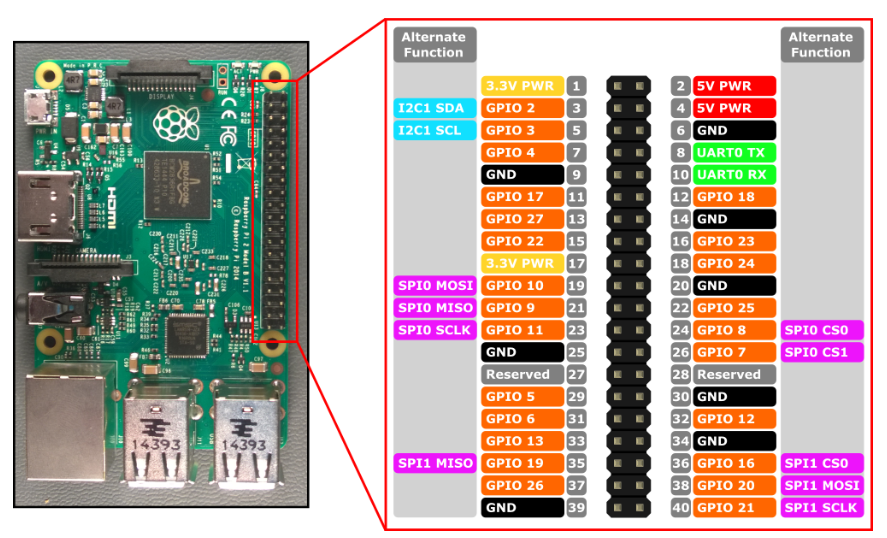
\includegraphics[width=0.7\textwidth]{images/esquemaRaspberry.png}
\caption{Diagrama de pines Raspberry-PI 3.}% 
\label{fig:pinesRaspberry}
\end{figure}


\section{Sistema operativo Raspbian}

Raspbian es un sistema operativo de código abierto basado en Debian, diseñado específicamente para funcionar en la placa R-Pi. Fue creado por el equipo de la Raspberry-Pi Foundation y se ha convertido en el sistema operativo más popular y ampliamente utilizado para la placa R-Pi.

Raspbian es un sistema operativo completo que incluye todas las herramientas y aplicaciones necesarias para realizar tareas típicas de una computadora, como navegar por la web, editar documentos, enviar correos electrónicos, programar y mucho más. La versión más reciente de Raspbian es Raspbian Buster, que se lanzó en 2019.

Entre las características de Raspbian se incluyen:

\begin{enumerate}
\item \textbf{Entorno de escritorio}: Raspbian viene con el entorno de escritorio LXDE, que es un entorno de escritorio ligero y eficiente que funciona muy bien en la placa R-Pi. También es posible instalar otros entornos de escritorio como XFCE, KDE y GNOME.
\item \textbf{Acceso a la terminal}: Además del entorno de escritorio, Raspbian también proporciona acceso a la terminal, lo que permite a los usuarios realizar tareas avanzadas de administración del sistema.
\item \textbf{Soporte para múltiples lenguajes de programación}: Raspbian incluye una gran cantidad de lenguajes de programación, incluyendo Python, Scratch, Ruby, C++, Java, entre otros. Esto hace que la placa R-Pi sea una excelente plataforma para la programación y el desarrollo de software.
\item \textbf{Software preinstalado}: Raspbian incluye una gran cantidad de software preinstalado, como el navegador web Chromium, la suite de ofimática LibreOffice, el reproductor de medios VLC, el cliente de correo electrónico Claws Mail, entre otros.
\item \textbf{Actualizaciones frecuentes}: La Raspberry-Pi Foundation actualiza regularmente Raspbian con parches de seguridad y mejoras de rendimiento.
\item \textbf{Fácil de instalar}: Raspbian se puede descargar gratuitamente desde el sitio web de la Raspberry-Pi Foundation y se puede instalar en la placa R-Pi utilizando una tarjeta SD.
\end{enumerate}


\section{Sensores}

Para este proyecto se utilizarán varios sensores conectados a la placa R-Pi, cada uno de ellos tiene ciertas características propias y utilidades las cuales serán descritas a continuación:

\subsection{MPU6000}

El MPU-6000 es un sensor de movimiento de seis ejes que combina un giroscopio de tres ejes y un acelerómetro de tres ejes en un solo chip. Este sensor es producido por la compañía InvenSense y ha sido utilizado en una gran variedad de aplicaciones, incluyendo drones, robots, consolas de juegos y otros sistemas de navegación.

El giroscopio de tres ejes mide la velocidad angular en cada uno de los tres ejes, permitiendo determinar la orientación y movimiento del objeto en el espacio. Por su parte, el acelerómetro de tres ejes mide la aceleración en cada uno de los tres ejes, lo que permite determinar la posición y velocidad de un objeto.

En cuanto a su conexión con la placa R-Pi, el MPU-6000 se puede conectar a través de un bus de comunicación utilizando protocolo SPI o I2C, lo que lo hace compatible con la mayoría de las placas R-Pi. 

El MPU6000 consta de 7 pines que se dividen en dos grupos: pines de alimentación y de comunicación. 

\begin{enumerate}
\item \textbf{Pines de alimentación}: El MPU-6000 requiere una alimentación de 3.3V, que se suministra a través de:

\begin{itemize}
\item \textit{VCC}: Suministro principal de alimentación y se conecta a una fuente de alimentación de 3.3V.
\item \textit{GND}: Conexión a la tierra de la fuente de alimentación.
\end{itemize}

\item \textbf{Pines de comunicación}: El MPU-6000 se comunica con otros dispositivos a través de los siguientes pines

\begin{itemize}
\item \textit{SCL}: Es el reloj del bus I2C y se utiliza para sincronizar la comunicación de datos.
\item \textit{SDA}: Es el canal de datos del bus I2C y se utiliza para transmitir y recibir datos.
\item \textit{AD0/SDO}: Se utiliza como dirección I2C para seleccionar el MPU-6000 si se están utilizando varios dispositivos I2C en la misma línea de bus. También puede utilizarse como salida de datos para la conexión SPI.
\item \textit{INT}: Se utiliza para enviar interrupciones al microcontrolador de la placa R-Pi para informar sobre cambios en los datos del sensor.
\end{itemize}
\end{enumerate}

En la Figura~\ref{fig:mpu6050} puede observarse el sensor MPU6050 junto con sus pines. 

\begin{figure}[h!]
\centering
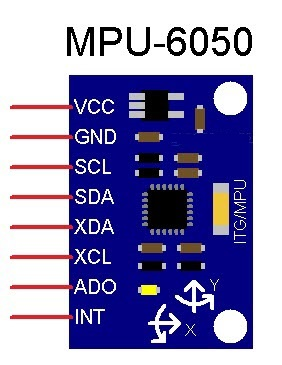
\includegraphics[width=0.3\textwidth]{images/mpu6050.jpg}
\caption[Sensor MPU6050]{Sensor MPU6050 junto con sus respectivos pines.}%
\label{fig:mpu6050}
\end{figure}



\subsection{HMC5983}
el HMC5983 es un sensor de campo magnético de tres ejes producido por la compañía Honeywell. Este sensor es utilizado para medir la intensidad y dirección del campo magnético en tres dimensiones. El HMC5983 cuenta con una resolución de 12 bits para cada eje, lo que le permite proporcionar mediciones precisas y confiables del campo magnético en entornos diversos. Además, cuenta con una alta estabilidad y una respuesta rápida, lo que lo hace adecuado para aplicaciones en las que es necesario detectar pequeñas variaciones en el campo magnético.

En cuanto a su conexión con la placa R-Pi, el HMC5983 se puede conectar a través de un bus de comunicación utilizando únicamente el protocolo I2C.

El sensor HMC5983 cuenta con 5 pines que se dividen en dos grupos: pines de alimentación y de comunicación. A continuación, se describen cada uno de ellos:

\begin{enumerate}
\item \textbf{Pines de alimentación}:  El HMC5983 requiere una alimentación de 3.3V, que se suministra a través de:

\begin{itemize}
\item \textit{VDD}: Es el suministro principal de alimentación y se conecta a una fuente de alimentación de 3.3V.
\item \textit{GND}: Se conecta a la tierra de la fuente de alimentación.
\end{itemize}

\item \textbf{Pines de comunicación}: El HMC5983 se comunica con otros dispositivos a través de:

\begin{itemize}
\item \textit{SCLK}: Es el reloj del bus I2C y se utiliza para sincronizar la comunicación de datos.
\item \textit{SDA}: Es el canal de datos del bus I2C y se utiliza para transmitir y recibir datos.
\item \textit{DRDY}: Se utiliza para enviar interrupciones al microcontrolador de la placa R-Pi para informar sobre cambios en los datos del sensor.
\end{itemize}
\end{enumerate}

En la Figura~\ref{fig:hmc5983} puede observarse el sensor HMC5983 junto con sus pines. 
\vspace{2mm}
\begin{figure}[h!]
\centering
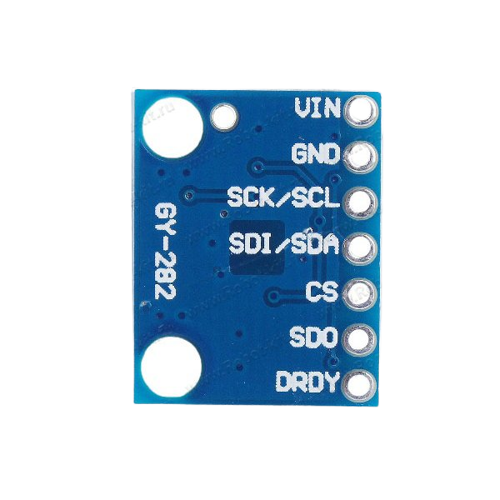
\includegraphics[width=0.4\textwidth]{images/hmc5983.png}
\caption [Sensor HMC5983]{Fotografía del Sensor HMC5983 en la que observan sus pines}
\label{fig:hmc5983}
\end{figure}

\subsection{HC-SR04}
El sensor de distancia HC-SR04 es un componente electrónico utilizado para medir la distancia entre el sensor y un objeto cercano. Se basa en el principio de la emisión y recepción de ondas ultrasónicas.

El HC-SR04 consta de dos partes principales: un transmisor y un receptor ultrasónico. El transmisor emite pulsos de alta frecuencia que no son audibles para los seres humanos. Estos pulsos se propagan en el aire en forma de ondas y cuando encuentran un objeto en su trayectoria, se reflejan hacia el sensor. El receptor del HC-SR04 recibe las ondas reflejadas y las convierte en señales eléctricas. El sensor utiliza un sistema de temporización para medir el tiempo que tarda en recibir la señal reflejada. A partir de esta medición de tiempo, se puede calcular la distancia entre el sensor y el objeto utilizando la fórmula de velocidad del sonido en el aire.

El HC-SR04 cuenta con 4 pines de conexión:
\begin{itemize}
\item \textit{VDD}: Suministra la alimentación al sensor, en este caso debe ser de 5V para su correcto funcionamiento.

\item \textit{Trig}: Se utiliza para iniciar la emisión de los pulsos electromagnéticos utilizados para medir la distancia.

\item \textit{Echo}: Encargado de recibir las señales ultrasónicas reflejadas en el objeto, aquellas que rebotan. Cuando el sensor recibe una señal reflejada, este pin se ocupa de producir un pulso cuya duración es proporcional a la distancia entre el sensor y el objeto.

\item \textit{GND}: Referencia a la tierra de la alimentación, debe estar conectado a un polo negativo para el correcto funcionamiento del sensor.
\end{itemize}

Es importante tener en cuenta que el rango de funcionamiento del HC-SR04 puede variar según las condiciones ambientales y la configuración del sistema. Sin embargo, generalmente puede medir distancias en un rango de varios centímetros hasta varios metros, aunque resulta mas fiable en entornos cerrados sin viento ni ruido y en distancias cortas.
El HC-SR04 es ampliamente utilizado en proyectos de electrónica y robótica, así como en aplicaciones de domótica. Se utiliza para tareas como detección de obstáculos, medición de distancias y sistemas de navegación entre otros. En la Figura~\ref{fig:ultrasonido} puede observarse el sensor HC-SR04 junto con sus pines. 

\vspace{2mm}
\begin{figure}[h!]
\centering
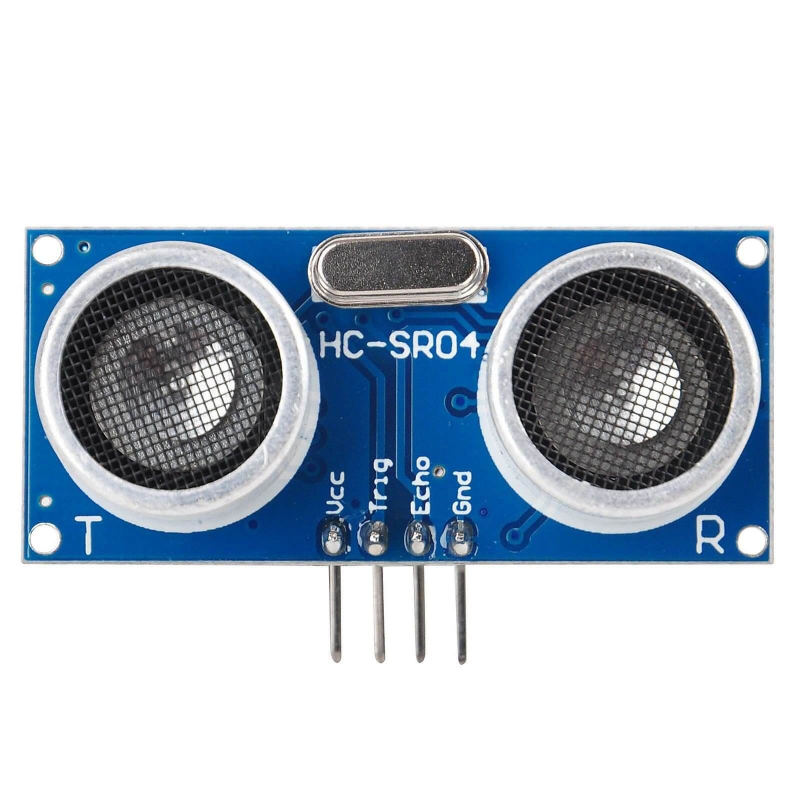
\includegraphics[scale=0.25]{images/HC_SR04}
\caption[Sensor HC-SR04]{Imagen del Sensor HC-SR04 con sus 4 pines observables}%
\label{fig:ultrasonido}
\end{figure}

\section{Apache JMeter}

\label{JMETER} JMeter es una herramienta de prueba de carga y rendimiento de código abierto desarrollada por Apache Software Foundation. Se utiliza principalmente para evaluar y medir el rendimiento de aplicaciones web y servidores, simulando un alto volumen de usuarios y analizando el comportamiento del sistema bajo diferentes cargas.

Algunas características importantes de JMeter son:

\begin{enumerate}
    \item \textbf{Pruebas de carga}: Permite simular un gran número de usuarios simultáneos accediendo a una aplicación web. Esto permite evaluar como responde la aplicación bajo cargas pesadas y determinar su capacidad de manejar un alto volumen de tráfico.
    \item \textbf{Pruebas de rendimiento}: Puede medir el rendimiento de una aplicación web al evaluar los tiempos de respuesta de las solicitudes y analizar métricas como la latencia, el tiempo de procesamiento del servidor y el de descarga de la página entre otros.
    \item \textbf{Escenarios de prueba flexibles}: Ofrece flexibilidad en la creación de escenarios de prueba. Se pueden configurar diferentes hilos de usuarios, establecer la secuencia de solicitudes HTTP y enviar solicitudes POST, GET, PUT y DELETE entre otras.
    \item \textbf{Análisis y generación de informes}: Proporciona informes y gráficos detallados sobre el rendimiento de la aplicación, incluyendo métricas como el tiempo de respuesta promedio, la tasa de errores, el rendimiento por solicitud y la distribución del tiempo de respuesta entre otros. Estos informes ayudan a identificar cuellos de botella y optimizar el rendimiento.
    \item \textbf{Soporte para diferentes protocolos}: Es compatible con varios protocolos, incluyendo HTTP, HTTPS, FTP, JDBC, LDAP, SOAP y JMS entre otros. Esto permite probar diferentes tipos de aplicaciones y servicios.
    \item \textbf{Extensibilidad}: Es altamente extensible y admite la creación de complementos personalizados para ampliar sus capacidades. Además, cuenta con una activa comunidad de usuarios que comparten complementos, scripts y soluciones a problemas comunes.
\end{enumerate}
